\chapter{Results}
\label{results}

\minitoc

In this chapter relevant articles gathered on ...

\newpage

\section{Introduction and Clarification}

\begin{table}[H]
\begin{center}
    \begin{tabular}{| p{5cm} | p{3.7cm} | p{1cm} | p{4cm} |}
    \hline
    \textbf{Article Name} & \textbf{Author(s)} & \textbf{Year} & \textbf{Keywords} \\ \hline
    Inter-team Coordination in Large-scale Globally Distributed Scrum: Do Scrum-of-Scrums Really Work? & Maria Paasivaara, Casper Lassenius, Ville T. Heikkilä & 2012 & Agile Software Development; Distributed Scrum; Global Software Engineering; Inter-team Coordination \\ \hline
    Communities of Practice in a Large Distributed Agile Software Development Organization – Case Ericsson & Maria Paasivaara, Casper Lassenius & 2014 & Communities of Practice; Large-scale Agile Software Development; Scaling Agile \\ \hline
    Operational Release Planning in Large-scale Scrum with Multiple Stakeholders – A Longitudinal Case Study at F-Secure Corporation & Ville T. Heikkilä, Maria Paasivaara, Kristian Rautiainen, Casper Lassenius, Towo Toivola, Janne Järvinen & 2015 & Agile Software Development; Scrum; Large Projects; Release Planning; Software Project Management \\ \hline
Towards a Governance Framework for Chains of Scrum Teams & Jan Vlietland, Hans van Vliet & 2015 & Agile; Chain of Scrum Teams; Coordination; Priority; Alignment; Predictability \\ \hline
    \end{tabular}
    \caption{Summary of articles used in this chapter.}
    \label{soauitc}
\end{center}
\end{table}

\begin{table}[H]
\begin{center}
    \begin{tabular}{| p{4cm} | p{8cm} |}
    \hline
    \textbf{Role} & \textbf{Description of role} \\ \hline
    Scrum master & \\ \hline
    Functional architect & \\ \hline
    Technical architect & \\ \hline
    Tester & \\ \hline
    Developer & \\ \hline
    \end{tabular}
    \caption{Team roles present in Scrum teams.}
    \label{trpist}
\end{center}
\end{table}

\begin{figure}[H]
\centering
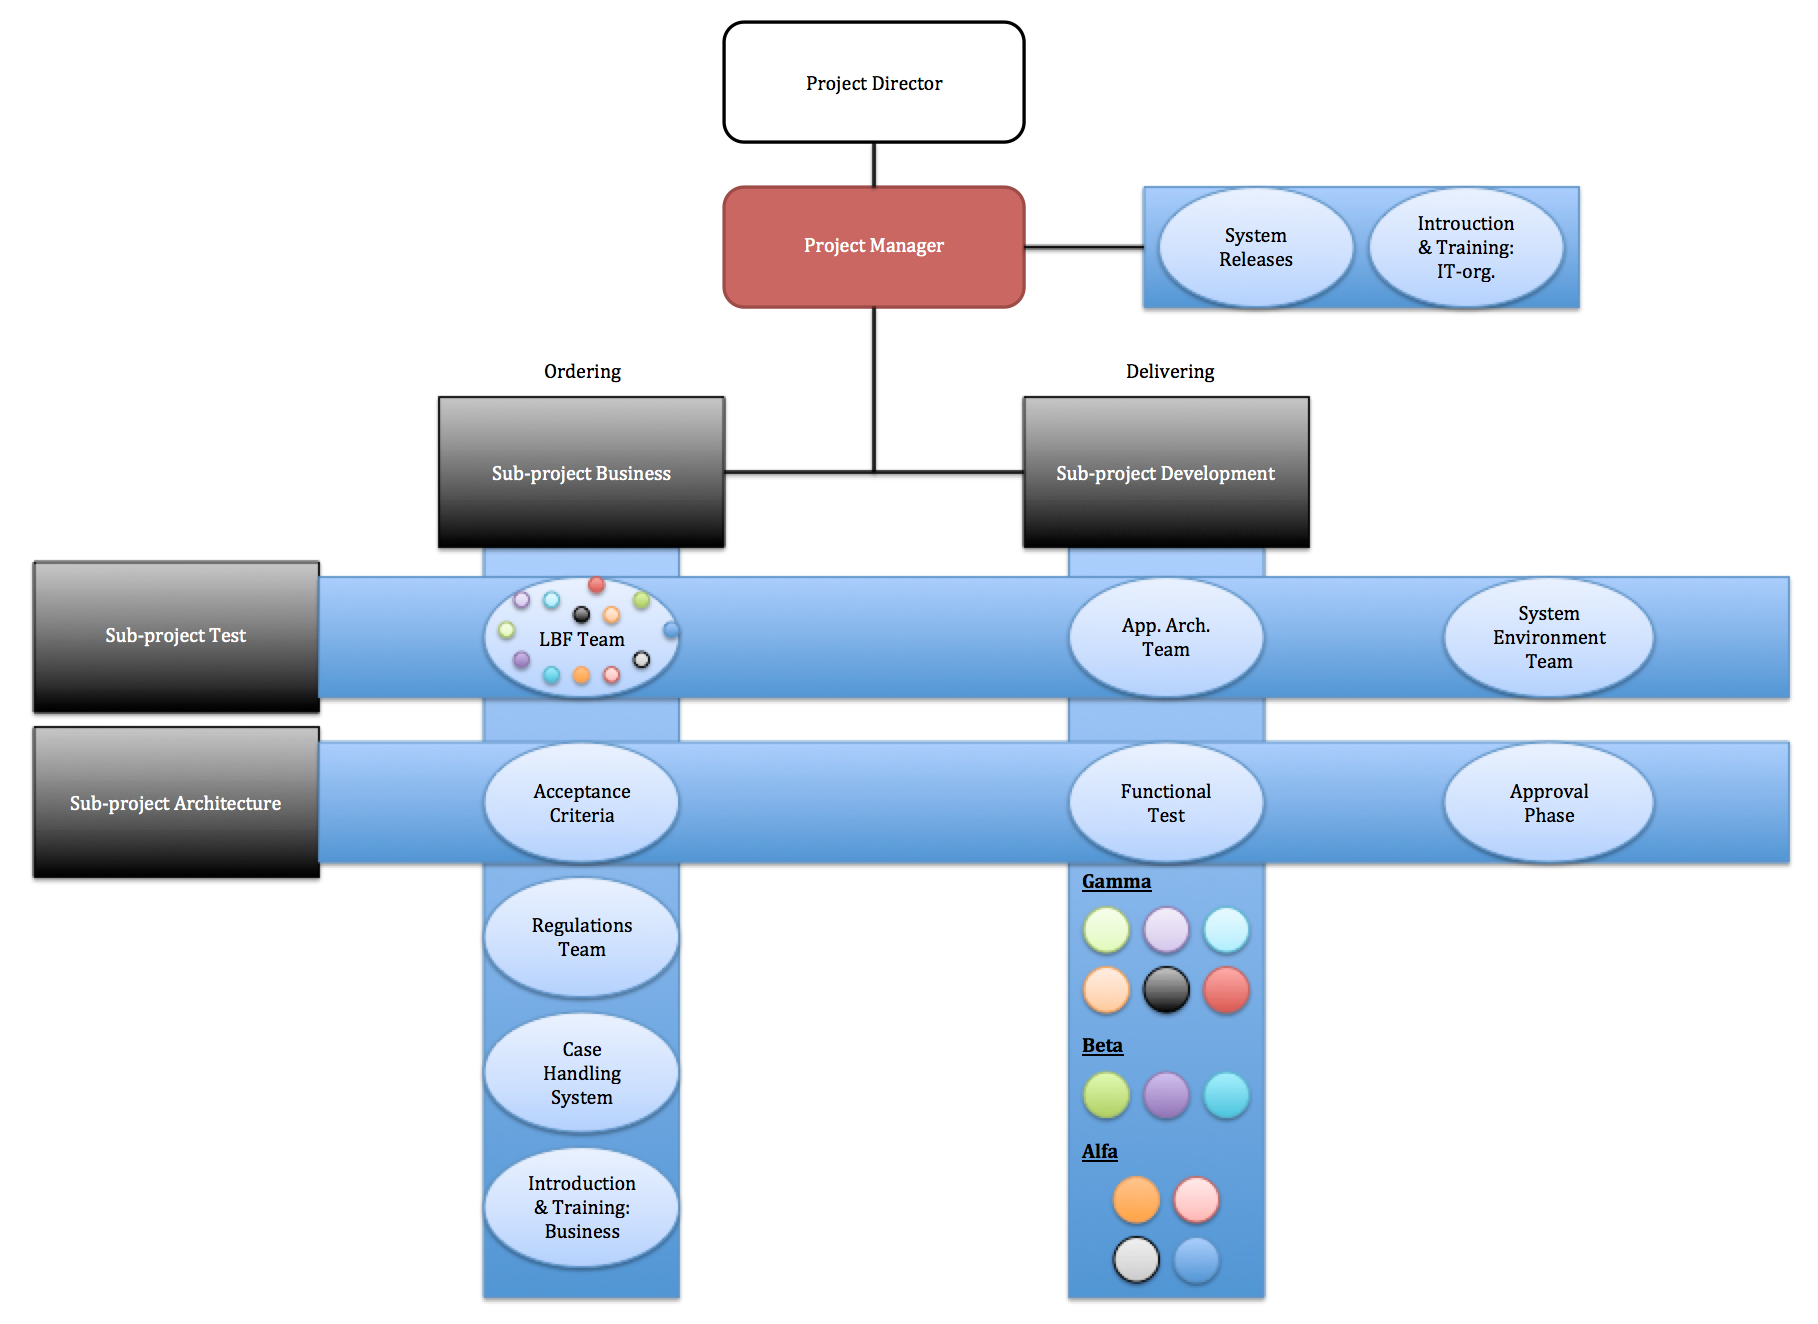
\includegraphics[trim = 40mm 0mm 7mm 0mm,width=180mm]{images/omega_organisation.png}
\caption{Omega-project's organisation.}
\label{omega}
\end{figure}

\begin{figure}[H]
\centering
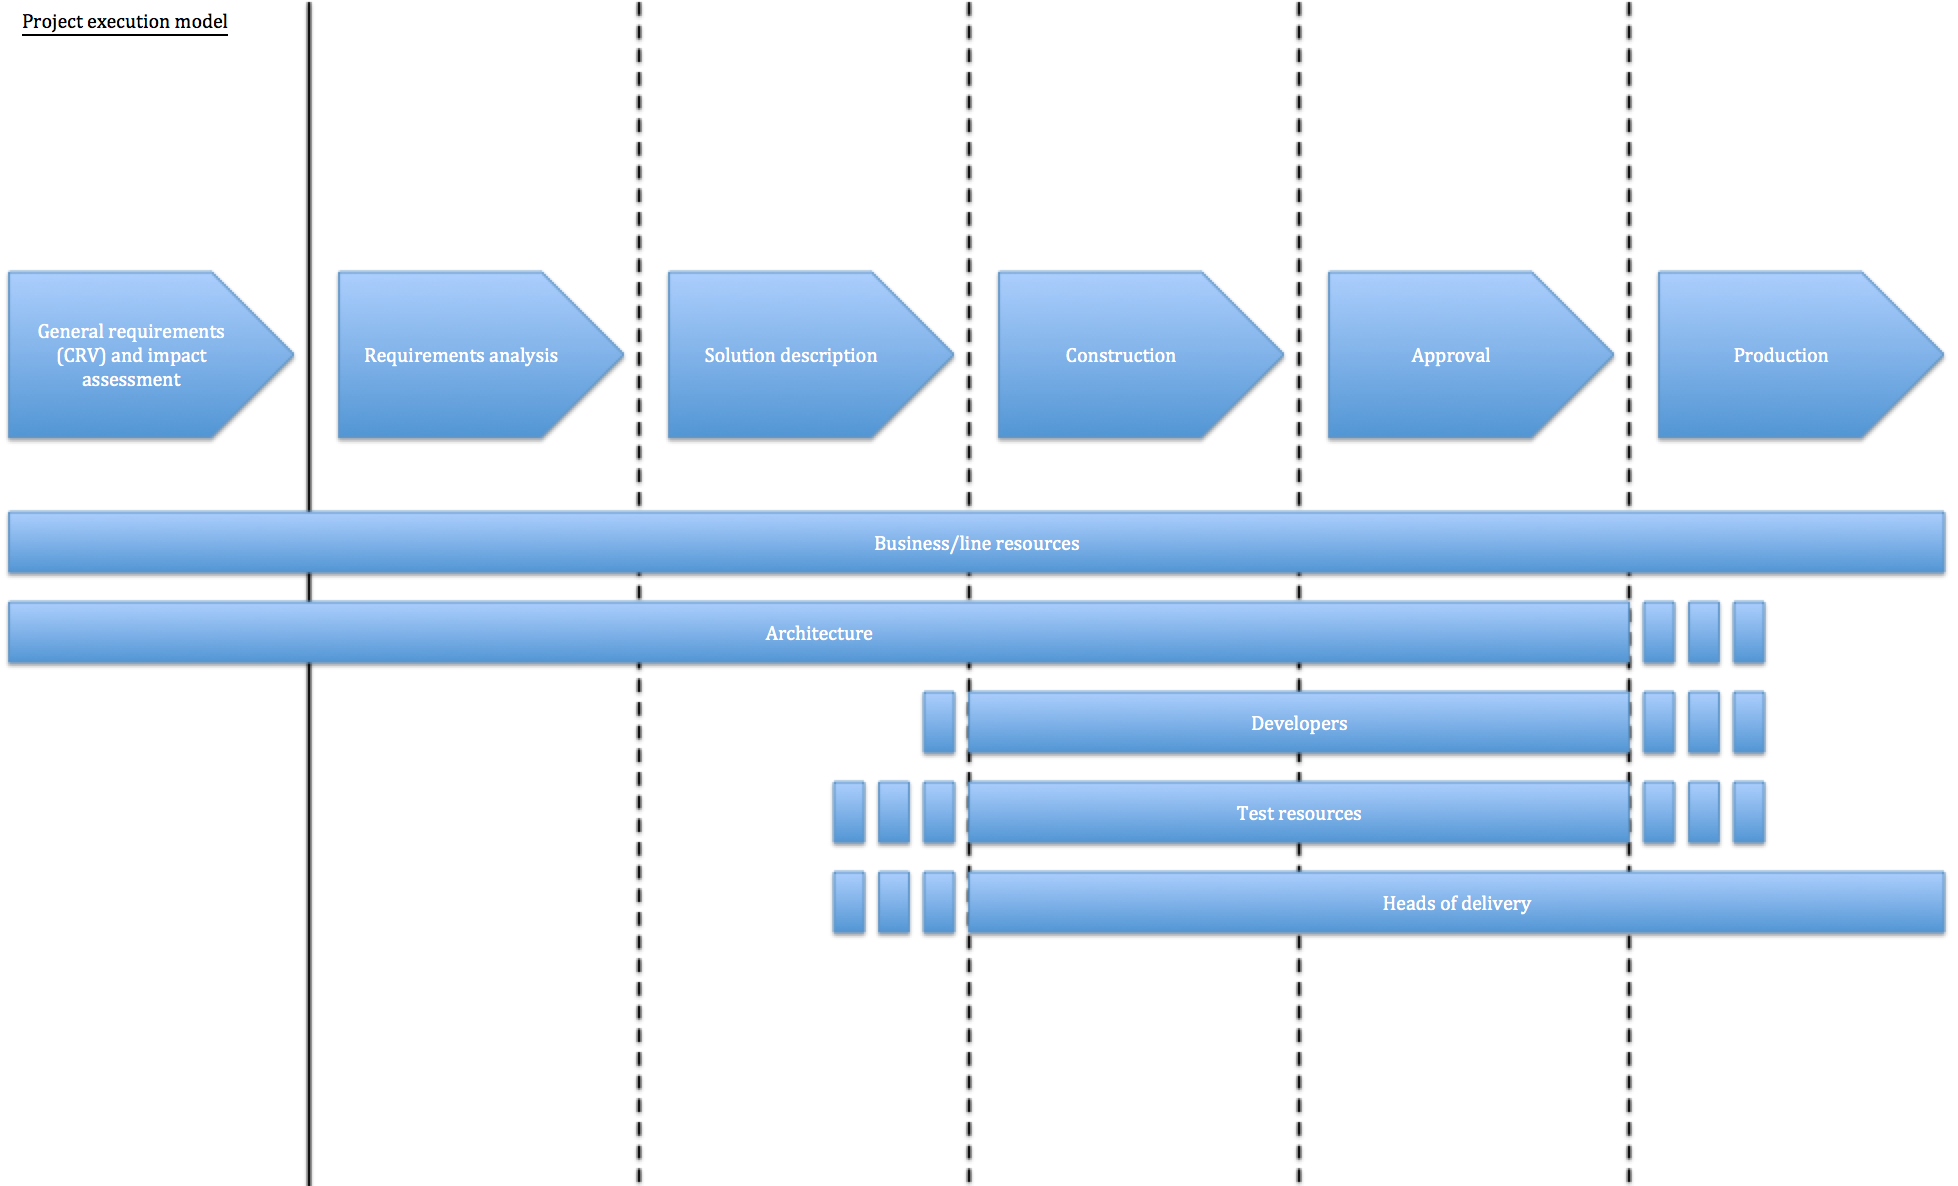
\includegraphics[trim = 40mm 0mm 7mm 0mm,width=180mm]{images/execution_model.png}
\caption{Project execution model.}
\label{project_execution}
\end{figure}

%På tvers: Metascrum, Planleggingsdag, Avhengighetsmøte, Front-end utviklernes møte, Wiki/Jira/Confluence, Uformelt, Open source/Lunch-seminar, Teknisk arkitektforum, Arkitekturråd, Forretning, QA, Demoer, Løsningsbeskrivelse, Testere (samme som QA?)
%Generelt: SoS. Stand-up. Tek-ark.-møte, Erfaringsutveksling, Planleggingsdag (tvers?), Leverandørmøte, Felles kaffepause, Team/Scrum-tavler + Whiteboard, Retrospektiv, Parprogrammering, Jevnlige møter (alfa s.10), "Teknisk hjørne", Jira-rom (tavler igjen), Planleggingsmøte (før planleggingsdag), Kontinuerlig planleggingsarbeid (avhengigheter), Iterasjonsoppstart, Utviklerforum (på tvers? Gamma s.9), Arkitektur (teknisk), Planleggingsmandag (ulike nivåer), Forhandlingsmøter+estimeringsmøter (på tvers?)
%Annet: Samme landskap, selvorganisering, tillit, problemer med team-følelse, rokkeringer på team og på plasseringer (av team), Beta/Alfa i Gamma-team, Prosjektledelse egen lokasjon (umiddelbar nærhet til teamene), 3 nivåer på produktsiden, sosial utenfor jobb (tillit igjen)